% https://github.com/abnt-latex/abntlatex
\documentclass[oneside]{abntlatex}

\usepackage[final]{pdfpages}
\usepackage{multibib}

\usepackage{threeparttable} % recommended IEEEtran package

\usepackage{multirow}
\usepackage{booktabs}

\usepackage{tabularx}

\usepackage{listings}

\usepackage{subcaption}

\renewcommand{\lstlistingname}{Código}
\renewcommand{\lstlistlistingname}{Lista de Códigos}

\lstdefinestyle{macrocode}{
    backgroundcolor  = \color{white},
    rulesepcolor     = \color{darkgray},
    commentstyle     = \color{gray},
    keywordstyle     = \color{blue}\bfseries,
    stringstyle      = \color{purple},
    basicstyle       = \ttfamily\footnotesize,
    showspaces       = false,
    showstringspaces = false,
    numbers          = left,
    tabsize          = 1,
    numberstyle      = \scriptsize,
    frame            = shadowbox,
    breaklines       = true,
    captionpos       = b,
}

\newcites{pub}{Publicações resultantes da Bolsa}

\title{Estudo de Duplicações em Subsistemas do Kernel Linux: Análise, Refatoração e Contribuições}
\author{Guilherme Ivo Bozi <guilherme.bozi@usp.br>}
\supervisor{Paulo Meirelles <paulormm@ime.usp.br>}
\university{%
Instituto de Matemática, Estatística e Ciência da Computação -- IME \\
Universidade de São Paulo -- USP \\
% bv.fapesp.br/pt/bolsas/233522/estudo-de-duplicacoes-em-subsistemas-do-kernel-linux-analise-refatoracao-e-contribuicoes/
Número do Processo FAPESP: 2025/22416-1%
}
\keywords{Manutenção de software, Software livre, Engenharia de software}
\date{%
Período de vigência da Bolsa: 01/11/2025 a 31/10/2026 \\
Período coberto pelo Relatório Científico: 01/11/2025 a 30/10/2026%
}

\makeatletter
\hypersetup{
    pdftitle={\@title},
    pdfauthor={\@author},
    pdfcreator={LaTeX2e with ABNT},
    pdfkeywords={\@keywords},
    hidelinks
}
\makeatother

\def\kernelauthor{42.412}
\def\kernelloc{28.130.130}

\hyphenation{Plotly ArKanjo WebGL Canvas amdgpu iio kernel Linux}

\def\boxtakeaway#1{
\noindent%
\fbox{\parbox{\dimexpr\textwidth-2\fboxsep-2\fboxrule\relax}{#1}}
\vspace{5pt}
}

\begin{document}
\pretext

% 2.1) Folha de rosto (1 página) contendo as seguintes informações: Título do
% projeto; Número do Processo FAPESP; Período de vigência; Período coberto pelo
% Relatório Científico em questão.
\backcover

% 2.2) Resumo do projeto proposto (até 2 páginas).
\begin{abstract}
A manutenção de sistemas computacionais de larga escala impõe desafios crescentes à engenharia de software. O \textbf{kernel Linux}, com \kernelauthor~contribuidores e \kernelloc~linhas de código\footnote{\texttt{Linux 7.2-rc2}; O número de linhas de código foi obtido utilizando a ferramenta \texttt{cloc}, considerando arquivos com extensão \texttt{.c}, \texttt{.h} e \texttt{.rs}. O número de contribuidores foi obtido a partir do histórico \texttt{git} utilizando o comando \texttt{git shortlog -sne -{}-all}.}, presente em servidores da internet, supercomputadores e sistemas operacionais modernos\cite{Corbet2017}, representa um ecossistema fundamental para a infraestrutura digital e para o avanço da ciência de dados. Este projeto de Iniciação Científica visa investigar a ocorrência de \textbf{código duplicado} no código-fonte do kernel Linux, com foco na identificação, análise e proposta de refatorações que melhorem sua manutenibilidade\cite{Alves2013}. A identificação dos códigos duplicados será conduzida por meio da ferramenta \texttt{ArKanjo}\cite{arcanjotese}\footnote{\url{https://gitlab.com/ccsl-usp/codev/arkanjo-tool}}, desenvolvida por nosso grupo de pesquisa\footnote{\url{https://gitlab.com/ccsl-usp/codev}} para detectar duplicações em nível de função, e utilizará uma abordagem qualitativa baseada em \textbf{observação participante}\cite{Seaman2008,Robson2016,Wen2021}. Como resultado, espera-se produzir contribuições práticas submetidas à comunidade do kernel Linux, bem como gerar evidências científicas sobre revisão e aceitação de \textit{patches} que removem duplicações, a partir da sistematização das experiências e interações realizadas durante o projeto.
\end{abstract}

\maintext
% 2.3) Realizações no período, se pertinente, referenciadas à lista de
% publicações do item 5 (até 10 páginas).

\part{Relatório Científico}

\section{Objetivos}

O objetivo central deste projeto é contribuir para a melhoria da qualidade do código do kernel Linux, identificando e mitigando duplicações de código em subsistemas selecionados. Como objetivos específicos:

\begin{itemize}
    \item Detectar duplicações em nível de função com o uso da ferramenta \texttt{ArKanjo};

    \item Analisar e selecionar duplicações para aplicar técnicas de refatoração, priorizando critérios de manutenibilidade;

    \item Propor e submeter \textit{patches} (contribuições) com refatorações para a comunidade do kernel Linux;

    \item Documentar o processo e as interações com a comunidade por meio de observação participante;

    \item Sistematizar as lições aprendidas e refletir sobre os aspectos sociotécnicos do processo de contribuição ao kernel Linux.
\end{itemize}

\section{Metodologia}\label{sec:metodologia}

Este projeto dá continuidade a estudos conduzidos pelo grupo de pesquisa entre 2024 e 2025\cite{arcanjo2025arkanjo,duplicationdry}, anteriores à vigência da bolsa, que utilizaram o \texttt{ArKanjo}~\cite{arcanjo2025arkanjo} para avaliar a viabilidade técnica e social da refatoração de duplicações no kernel Linux. Em 2026, os procedimentos foram replicados com novos participantes. A abordagem é um estudo multimétodo de caráter etnográfico, que combina detecção automatizada de duplicações, observação participante\cite{Seaman2008,Robson2016,Wen2021} e um estudo com novos contribuidores (estudantes) do kernel Linux.

\subsection{Subsistemas estudados}

O estudo concentrou-se nos subsistemas \texttt{\textbf{amdgpu}} e \texttt{\textbf{iio}}. O \texttt{amdgpu}, \textit{driver} das GPUs AMD, tem arquitetura em camadas, com código genérico nas camadas superiores e código específico de hardware nas inferiores, frequentemente compartilhado entre dispositivos\cite{Wang2011}. Isso favorece a cópia de código entre gerações de hardware\cite{duplicationdry}. O \texttt{iio} (\textit{Industrial I/O}) reúne \textit{drivers} de conversores analógico-digitais e digital-analógicos e foi escolhido por ser considerado uma porta de entrada acessível para novos contribuidores\cite{duplicationdry}. A distribuição das duplicações nos dois subsistemas é apresentada na Seção~\ref{sec:visualizacoes}.

\subsection{Procedimentos}

O estudo foi organizado em três etapas:

\begin{enumerate}
    \item \textbf{Identificação e seleção}

    Detecção de duplicações em nível de função com o \texttt{ArKanjo}, com similaridade de 90\% e 100\%, seguida da análise de seu potencial de refatoração.

    \item \textbf{Implementação e submissão}

    Desenvolvimento e submissão dos \textit{patches} para mitigar as duplicações selecionadas, incluindo a interação com os mantenedores e a realização dos ajustes solicitados.

    \item \textbf{Análise dos \textit{patches}}

    Identificação, a partir das revisões dos mantenedores, de \textit{takeaways} sobre a aceitação e a rejeição das propostas, considerando os \textit{patches} de 2026.
\end{enumerate}

\subsection{Coleta de dados}\label{sec:coleta-dados}

% 40 de graduacao; 16 de pos; 56 total; citar que é graduacao e pos

Por meio de \textbf{observação participante}, o bolsista interagiu com a comunidade e submeteu \textit{patches} para contribuir com os subsistemas analisados. Além disso, conduziu um \textbf{estudo com participantes} envolvendo alunos da disciplina MAC0470/5856 -- Desenvolvimento de Software Livre (USP, 2026/1)\footnote{\url{https://uspdigital.usp.br/jupiterweb/obterDisciplina?sgldis=MAC0470}}, que contou com 56 alunos matriculados, sendo 40 de graduação e 16 de pós-graduação. Desse total, 22 alunos (39,3\%) participaram das atividades de deduplicação de código, organizados em 12 grupos. A disciplina foi organizada em duas fases: na primeira, os estudantes atuaram como contribuidores do kernel Linux, utilizando os resultados de detecção do \texttt{ArKanjo} para identificar, refatorar e submeter \textit{patches} relacionados a duplicação de código; na segunda, os grupos escolheram um projeto de software livre qualquer para contribuir, e alguns optaram pelo próprio \texttt{ArKanjo}.

Os demais 34 alunos, durante a primeira fase, escolheram outros temas de contribuição ao kernel Linux. Essas contribuições não fazem parte da análise deste relatório.

\section{Atividades realizadas e resultados}

\subsection{Análise: detecção e seleção de duplicações}\label{sec:deteccao}

A detecção, no âmbito da disciplina, foi realizada com o \texttt{ArKanjo} apenas nos subsistemas \texttt{amdgpu} e \texttt{iio}, com similaridade de 90\% e 100\%, sendo cada duplicação avaliada manualmente quanto ao potencial de refatoração. Desse processo foram propostas 13 duplicações aos alunos da disciplina MAC0470/5856. Os grupos selecionaram 12 duplicações para realizar refatorações. Essa contagem não inclui as duplicações trabalhadas pelo bolsista (Seção~\ref{sec:refatoracao}).

\subsection{Visualizações: exploração de duplicações de código}\label{sec:visualizacoes}

Para facilitar a exploração dos resultados de detecção de duplicações produzidos pelo \texttt{ArKanjo}, estão sendo desenvolvidas, pelo bolsista, visualizações interativas no contexto da disciplina MAC0214 -- Atividade Curricular em Cultura e Extensão (USP, 2026/2)\footnote{\url{https://uspdigital.usp.br/jupiterweb/obterDisciplina?sgldis=mac0214}}. Diferente da detecção usada na seleção de \textit{patches}, as visualizações foram geradas sobre o kernel Linux completo. A Figura~\ref{fig:treemap} apresenta uma visualização hierárquica (\textit{treemap}) do kernel, com os subsistemas \texttt{amdgpu} e \texttt{iio} em destaque, mostrando a distribuição das duplicações entre suas pastas. A Figura~\ref{fig:heb} apresenta uma visualização baseada em \textit{Hierarchical Edge Bundling} (HEB), na qual as conexões representam relações de duplicação entre arquivos.

\begin{figure}[htbp]
    \centering
    \begin{subfigure}[t]{0.48\textwidth}
        \centering
        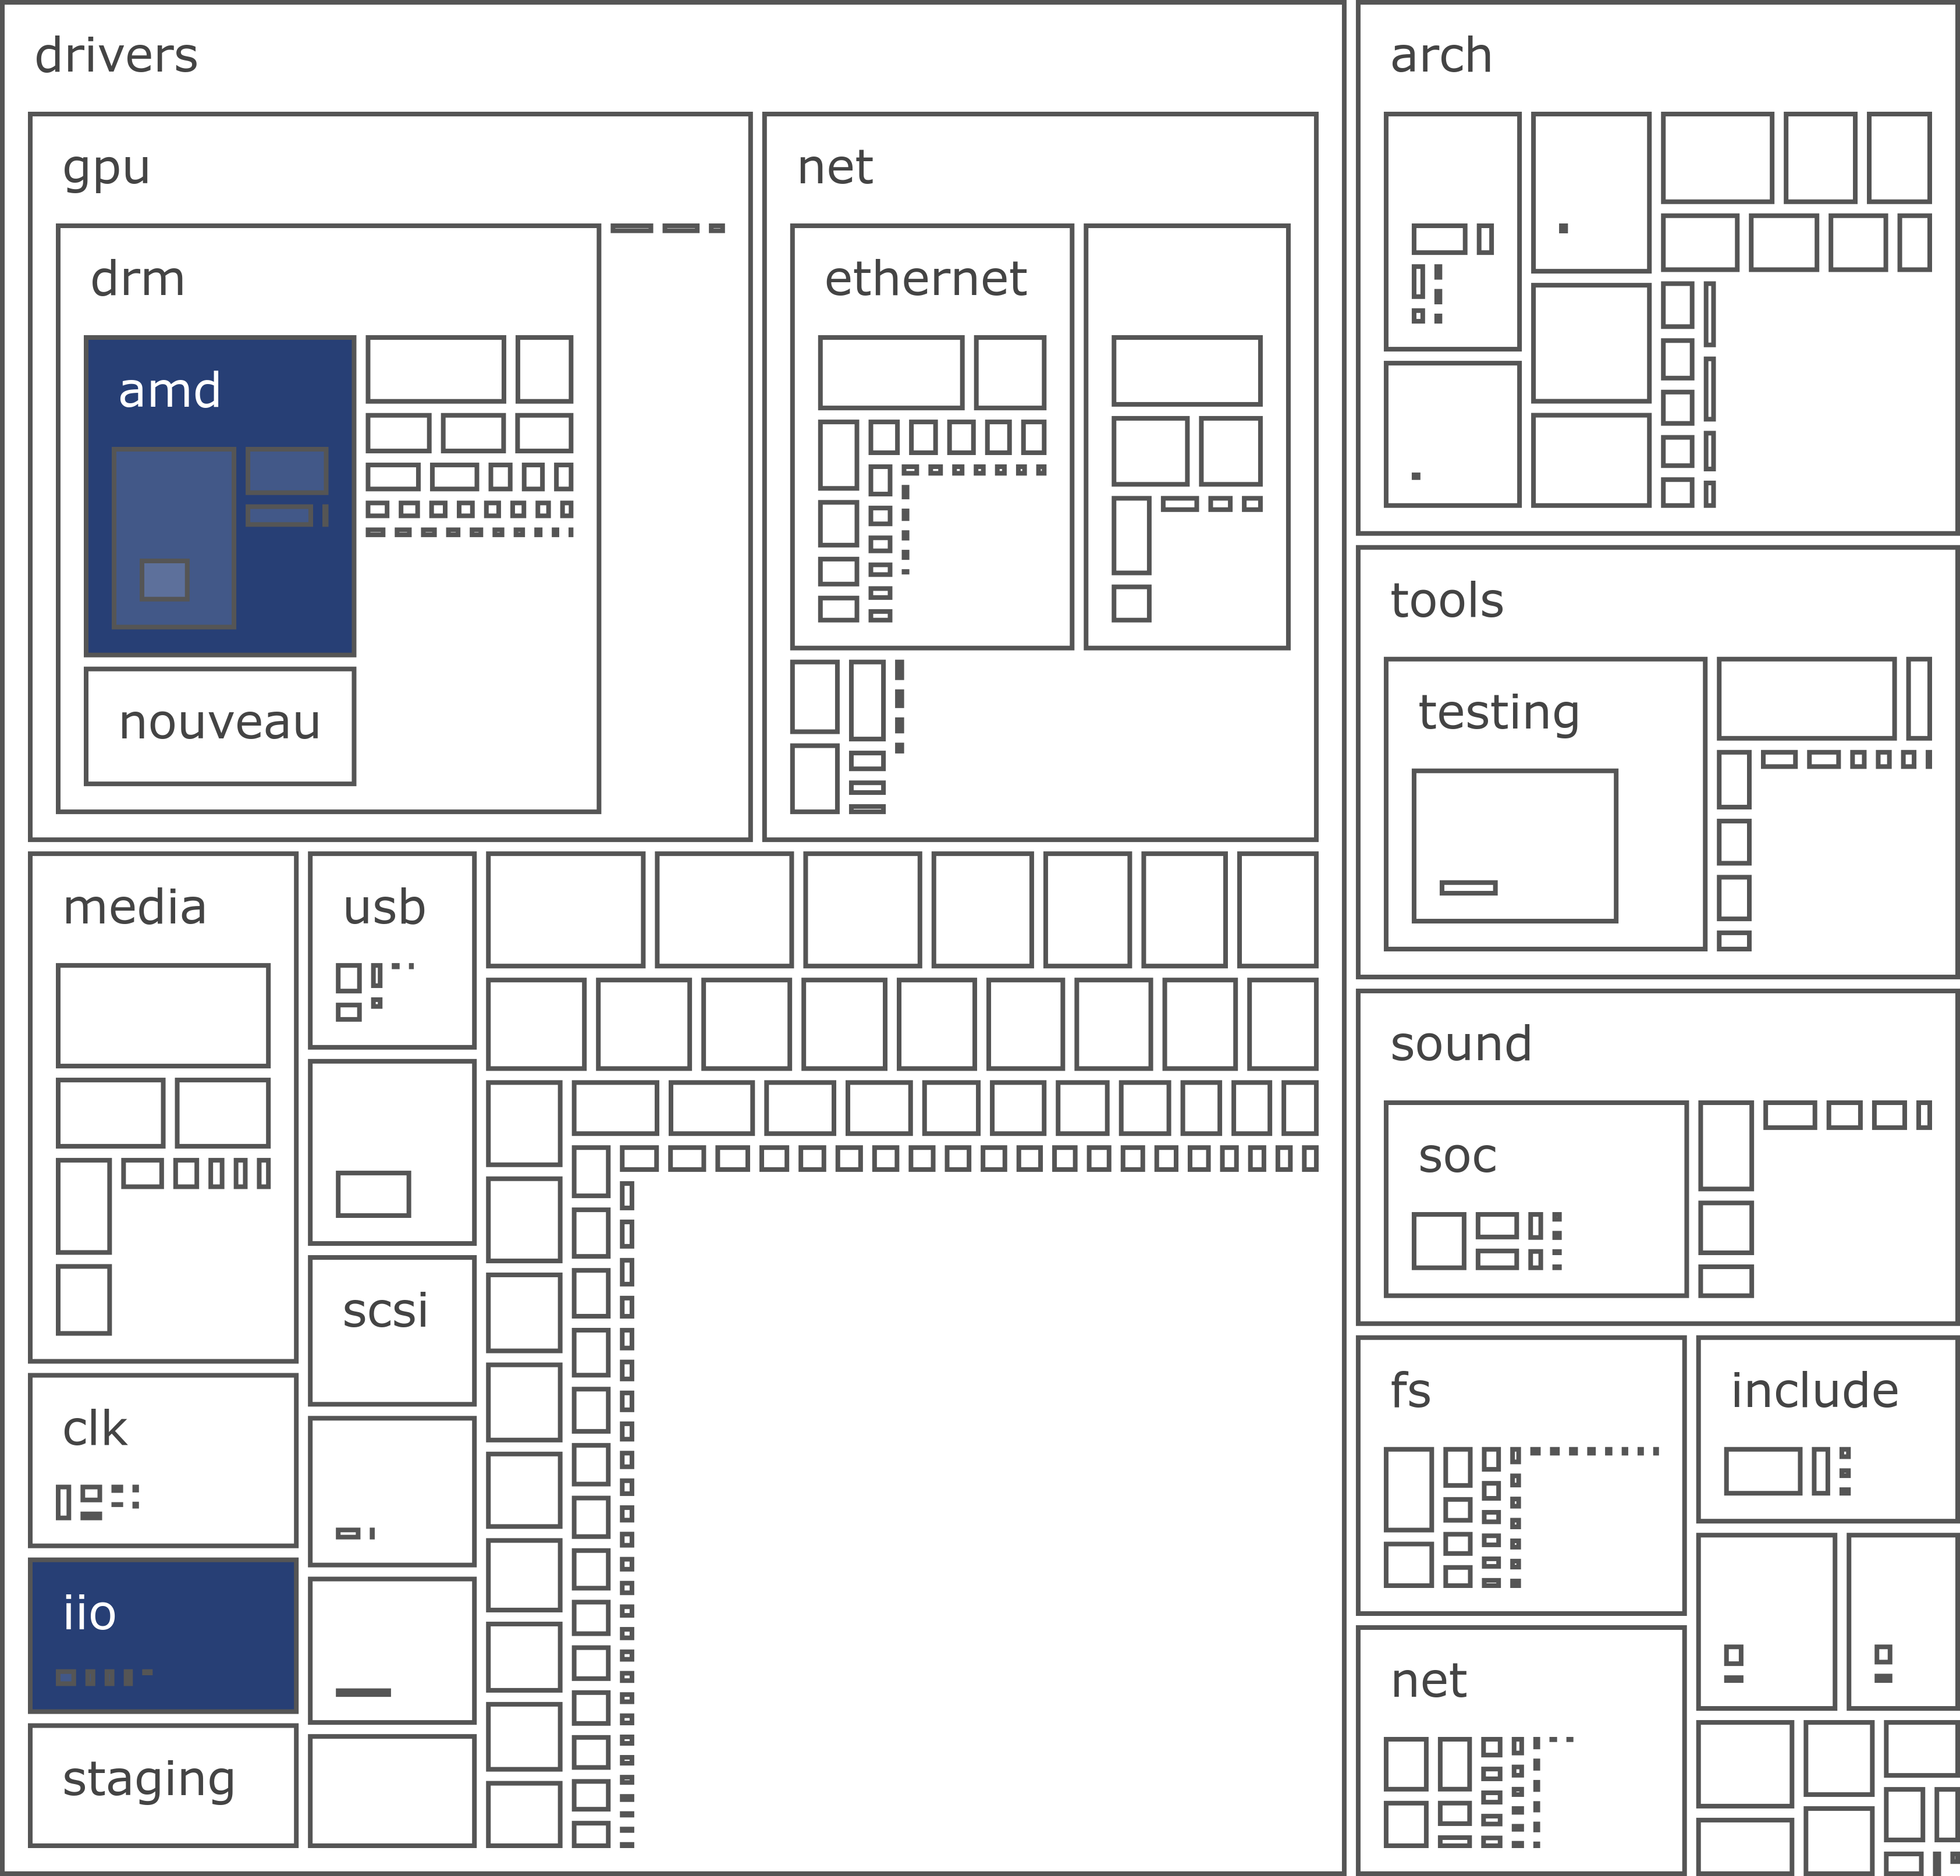
\includegraphics[width=\textwidth]{figures/treemap.png}
        \caption{Concentração de duplicações nas pastas dos subsistemas analisados em destaque. Renderização de uma visualização interativa implementada usando Plotly.}
        \label{fig:treemap}
    \end{subfigure}
    \hfill
    \begin{subfigure}[t]{0.48\textwidth}
        \centering
        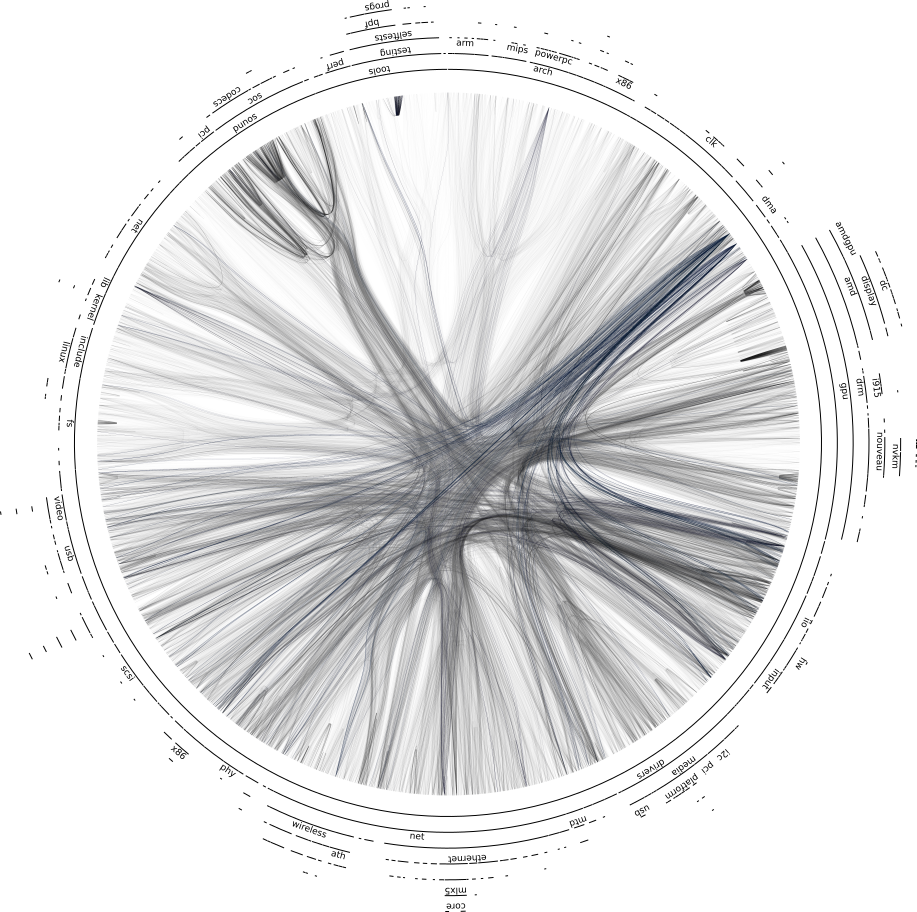
\includegraphics[width=\textwidth]{figures/heb.png}
        \caption{Cada aresta liga dois arquivos com funções duplicadas. Renderização de uma visualização interativa implementada com WebGL2 ou Canvas2d.\footnotemark}
        \label{fig:heb}
    \end{subfigure}
    \caption{Visualizações de duplicações de função detectadas pelo  \texttt{ArKanjo} no kernel Linux, com similaridade de 100\%.}
\end{figure}

\footnotetext{\url{https://guilhermeivo.com.br/duplication-viz/}}

\subsection{Refatoração: \textit{patches} e interação com a comunidade}\label{sec:refatoracao}

%3.3 Refatoração: patches e interação com a comunidade
%(observacao participante )

Por meio de observação participante, o bolsista investigou o processo de remoção de duplicações de código nos subsistemas \texttt{amdgpu} e \texttt{iio} do kernel Linux, desde a identificação de oportunidades de refatoração até a revisão das propostas pelos mantenedores.

No período, o bolsista atuou como contribuidor, submetendo 4 séries de \textit{patches}, das quais três foram aceitos e integrados ao kernel, enquanto um permaneceu sem resposta dos mantenedores (as 4 primeiras contribuições GID~0 na Tabela~\ref{tab:patches}, onde a quinta contribuição GID~0 foi desenvolvida por um membro do grupo de pesquisa externo à disciplina), e, nas contribuições dos grupos, como mentor.

Sua principal contribuição foi uma série de nove \textit{patches} ao \texttt{amdgpu} (+1274/-2035, GID~0 na Tabela~\ref{tab:patches})\footnote{\url{https://lore.kernel.org/all/20260512190019.228440-1-guilherme.bozi@usp.br/}}, que substituiu estruturas \texttt{switch-case} de tradução de GPIO por tabelas de consulta com funções auxiliares genéricas, com redução líquida de 761 linhas; a série foi aceita já na primeira versão. Em outra contribuição, ao tentar modernizar o \textit{driver} \texttt{xilinx-ams} do \texttt{iio}\footnote{\url{https://lore.kernel.org/all/20260513003503.339418-1-guilherme.bozi@usp.br/}}, e remover duplicações, o bolsista identificou e corrigiu um acesso fora dos limites (\textit{out-of-bounds}), falha à qual foi atribuído o CVE-2026-72480\footnote{\url{https://www.cve.org/CVERecord/?id=CVE-2026-72480}}.

Como parte do fluxo de desenvolvimento estabelecido pelo grupo de pesquisa, os \textit{patches} eram submetidos inicialmente a uma instância interna do Lore do IME-USP\footnote{\url{https://lore.kernel.ime.usp.br/kernel.ime/}}, onde um sistema de integração contínua (CI) executava verificações automatizadas antes do envio às listas de discussão oficiais do kernel Linux. Essa etapa permitia identificar problemas antes da submissão à comunidade e integrava o processo de preparação e validação das contribuições.

As interações com os mantenedores são analisadas na Seção~\ref{sec:mentoria}, que apresenta os \textit{patches} submetidos no período e os relaciona aos \textit{takeaways} do estudo anterior do grupo\cite{duplicationdry}.

\subsubsection{Mentoria e avaliação dos \textit{patches}}\label{sec:mentoria}

%3.4. Mentoria e análise do patches do estudantes
%(observacao participante as observer)
%citar o CI

Como mentor, o bolsista indicou duplicações candidatas aos grupos, auxiliou na resolução dos problemas, na submissão e no atendimento às revisões, e revisou \textit{patches} dos grupos na instância interna do Lore antes do envio às listas oficiais.

Foram submetidas 17 séries de \textit{patches} para remoção de duplicações nos subsistemas \texttt{amdgpu} e \texttt{iio} do kernel Linux. Dessas, 4 foram submetidas pelo bolsista, 1 foi desenvolvido por um pesquisador do grupo externo à disciplina e 12 foram elaborados pelos estudantes da disciplina MAC0470/5856, organizados em 12 grupos. Das 17 séries de \textit{patches}, 10 foram aceitas e integradas ao kernel (59\%), quatro foram rejeitadas, dois permaneceram sem resposta dos mantenedores e uma foi abandonada durante o desenvolvimento.\footnote{O resumo do SIICUSP (Apêndice~\ref{apx:publicacoes-resultantes-da-bolsa}) mostra dados de uma data anterior a este relatório: 8 aceitos, 4 em revisão e 5 não incorporados, com remoção líquida de 1.096 linhas. O pôster apresentado já traz os números atuais.} A Tabela~\ref{tab:patches} apresenta o estado de cada contribuição, o subsistema envolvido, o limiar de similaridade considerado, os \textit{takeaways} associados e as linhas adicionadas e removidas.

\begin{table}[!ht]
\centering
\small\linespread{1.0}\selectfont
\begin{threeparttable}
    \caption{Resumo das contribuições das séries de \textit{patches} de deduplicação ao kernel Linux\tnote{a}.}
    \label{tab:patches}
\begin{tabularx}{\textwidth}{ c c c X l c }
\toprule
\textbf{GID} & \textbf{SS} & \textbf{SML} & \textbf{Series Status} & \textbf{Takeaway} & \textbf{Diff} \\
\midrule
\multirow[t]{5}{*}{0} & AMD & 100\% & No response & -- & \texttt{+86/-114} \\
  & IIO & 100\% & Accepted (v1), Merged & -- & \texttt{+15/-32} \\
  & IIO & 100\% & Accepted (v4), Merged & -- & \texttt{+71/-119} \\
  & AMD & 90\% & Accepted (v1), Merged & T2 & \texttt{+1274/-2035} \\
  & AMD & 100\% & Accepted (v3), Merged & T3, T5 & \texttt{+41/-124} \\
1 & AMD & 100\% & Accepted (v2), Merged & T1, T5 & \texttt{+12/-61} \\
2 & AMD & 100\% & Accepted (v2), Merged & T1 & \texttt{+13/-42} \\
3 & AMD & 100\% & Rejected (v1) & T1, T5 & \texttt{+61/-94} \\
4 & AMD & 100\% & Accepted (v4), Merged & T1 & \texttt{+56/-102} \\
5 & IIO & 100\% & Accepted (v4), Merged & T2 & \texttt{+29/-66} \\
6 & IIO & 100\% & Accepted (v4), Merged & T2, T3 & \texttt{+42/-88} \\
7 & AMD & 100\% & Rejected (v1) & T1 & \texttt{+131/-190} \\
8 & AMD & 100\% & No response & -- & \texttt{+42/-75} \\
9 & AMD & 100\% & Accepted (v6), Merged & T1, T5 & \texttt{+66/-89} \\
10 & AMD & 90\% & Rejected (v1) & T1, T5 & \texttt{+47/-124} \\
11 & IIO & 90\% & Rejected (v1) & T2, T3 & \texttt{+63/-62} \\
12 & IIO & 90\% & Dropped (v2) & T2 & \texttt{+42/-60} \\
\bottomrule
\end{tabularx}
\begin{tablenotes}[flushleft]
\footnotesize
\item[a] GID: grupo (0: bolsista e pesquisador do grupo; 1--12: grupos da disciplina); SS: subsistema (AMD: \texttt{amdgpu}; IIO: \texttt{iio}); SML: limiar de similaridade; Status: situação da série (Accepted: aprovada; Merged: integrada; Rejected; Dropped: abandonada; No response), com a versão (vN) em que foi encerrada; Diff: linhas adicionadas e removidas.
\end{tablenotes}
\end{threeparttable}
\end{table}

As 10 séries de \textit{patches} integradas totalizaram 1.619 linhas adicionadas e 2.758 removidas, resultando em uma redução líquida de 1.139 linhas. Uma contribuição ao subsistema \texttt{amdgpu}, com 1.274 linhas adicionadas e 2.035 removidas, correspondeu a uma redução líquida de 761 linhas.

Para analisar as decisões dos mantenedores, foram considerados os quatro \textit{takeaways} identificados no estudo anterior do grupo\cite{duplicationdry}. Esse estudo examinou 13 contribuições de deduplicação nos subsistemas \texttt{amdgpu} e \texttt{iio}, das quais oito foram aceitas (62\%). Os \textit{takeaways} abordam o \textit{driver forking} (T1), a priorização da legibilidade (T2), o custo de integração das mudanças (T3) e o impacto no desempenho (T4).

\vspace{20pt}

\boxtakeaway{\textbf{Takeaway T1 (Driver Forking):} \textit{Driver developers do not necessarily view duplicated code negatively, often consciously cloning entire drivers for many reasons; however, sometimes such duplications are explicitly acknowledged as technical debt, and their repayments are accepted when perceived as safe and stable.}}

\boxtakeaway{\textbf{Takeaway T2 (Readability):} \textit{Maintainers prioritized readability over removing duplication across many contexts. Accepting debt from duplication may be worth it if it results in easier-to-read, more understandable code. Nevertheless, the criteria used to accept or reject similar repayments that affect readability require deeper investigation.}}

\boxtakeaway{\textbf{Takeaway T3 (Integration Overhead):} \textit{Maintainers may decline to accept a duplication repayment if it is not considered impactful enough, because simply integrating it into the Linux upstream incurs considerable debt principal.}}

\boxtakeaway{\textbf{Takeaway T4 (Performance):} \textit{Interactions with maintainers hinted that duplications can be forgiven if they improve performance in contexts where resources are limited. In these scenarios, avoiding performance debt is prioritized.}}

A análise dos \textit{patches} submetidos no período também levou à formulação de um quinto \textit{takeaway}, apresentado nas apresentações orais do SIICUSP~2026~\citepub{bozi2026siicusp}. O T5 foi derivado da leitura das discussões de revisão dos patches de 2026. O bolsista leu as threads de cada contribuição e registrou as justificativas dos mantenedores para aceitar, redirecionar ou rejeitar a proposta, verificando se cada uma se enquadrava em T1--T4. A formulação do T5 e sua associação aos patches foram então discutidas e validadas com o grupo de pesquisa.

\vspace{20pt}
\boxtakeaway{\textbf{Takeaway T5 (Abstraction Scope):} \textit{Mantenedores podem rejeitar ou redirecionar uma remoção de duplicação quando o código duplicado não compartilha uma barreira de abstração adequada. Consolidá-lo em uma camada compartilhada pode ser considerado inadequado quando o comportamento não se aplica de modo uniforme a todos os componentes atendidos por essa camada.}}
\vspace{10pt}

O T5, relacionado ao escopo da abstração, foi associado a cinco das 17 séries de \textit{patches}: 3 foram aceitos após alterações na proposta durante o processo de revisão, e 2 foram rejeitados (Tabela~\ref{tab:patches}). Em um dos casos considerados na formulação desse \textit{takeaway}, o mantenedor comentou:

\begin{quote}
\textit{``Please don't when they are functional identical then move them a layer up instead of messing up the backends.''} (GID 0, Tabela \ref{tab:patches})
\end{quote}

Entre os \textit{patches} analisados no período, T1, T2 e T3 foram associados a contribuições da tabela, enquanto T4 não foi associado a nenhum dos casos. O T5 acrescenta à análise a questão do escopo da abstração, identificada a partir das revisões das contribuições submetidas em 2026.

\subsection{Contribuições: ArKanjo e \textit{dataset}}

Durante a bolsa, o bolsista implementou no \texttt{ArKanjo} melhorias arquiteturais e novas funcionalidades, entre elas:

\begingroup
\renewcommand{\labelenumi}{(\alph{enumi})}
\begin{enumerate}
\item migração do \textit{parser} manual para o \texttt{Tree-sitter}\footnote{\url{https://tree-sitter.github.io/tree-sitter/}}, que facilita o suporte a novas linguagens, como Rust e a análise do código;
\item uso de árvores sintáticas abstratas (ASTs) durante o \textit{pipeline} de análise;
\item um sistema de comandos mais modular, que reduz o esforço para contribuições externas;
\item e saídas estruturadas (JSON e \textit{templates}, exemplo de uso no Código~\ref{lbl:code-explorer}), para integração com \textit{scripts}.
\end{enumerate}
\endgroup

\vspace{20pt}

\begin{lstlisting}[style=macrocode,numbers=none,label=lbl:code-explorer,language=bash,morekeywords={arkanjo},caption={Exploração das duplicações analisadas usando \texttt{-{}-template} como argumento.}]
arkanjo explorer --template "{func_a:function} ~ {func_b:function} ({duplicated_lines:number} lines)"
\end{lstlisting}

Além dessas, outras contribuições foram enviadas, por alguns grupos de estudantes, para o \texttt{ArKanjo}, durante a segunda fase da disciplina MAC0470/5856 (Seção~\ref{sec:metodologia}). Foram identificadas contribuições de 6 grupos, esse conjunto é distinto dos 22 alunos que atuaram na deduplicação de código do kernel (Seção~\ref{sec:coleta-dados}), alguns estudantes participaram das duas fases. Entre as contribuições, um grupo desenvolveu um método baseado em \textit{embeddings} para detecção de clones Type-3 e Type-4. Para avaliar esse método, o bolsista implementou, durante a disciplina MAC0215 -- Atividade Curricular em Pesquisa (USP, 2026/1)\footnote{\url{https://uspdigital.usp.br/jupiterweb/obterDisciplina?sgldis=mac0215}}, um comando de \textit{benchmark} no \texttt{ArKanjo}, com adaptadores para o BigCloneBench\cite{svajlenko2014bigclonebench} e o POJ-104\cite{mou2016convolutional} (Código~\ref{lbl:code-bench}), e o comparou com os métodos de AST linearizada e TF-IDF. Nos subconjuntos avaliados, os métodos de AST linearizada e de \textit{embeddings} apresentaram \textit{recall} superior ao do TF-IDF em clones Type-3 e Type-4, enquanto o método de \textit{embeddings} obteve o maior F1-Score agregado, mas com maior tempo de execução. Os resultados detalhados (\textit{recall}, F1-Score e tempo de execução por método e por \textit{benchmark}) estão no relatório produzido para a disciplina MAC0215\cite{bozi2026mac0215} e no vídeo de apresentação\footnote{\url{https://youtu.be/e_RUDak7OtA}}, material do primeiro semestre de 2026, anterior ao fechamento dos números deste relatório. A avaliação foi realizada nos subconjuntos dos \textit{benchmarks}; não foi possível avaliá-los diretamente no kernel Linux, que não possui rótulos de referência.

\vspace{20pt}
\begin{lstlisting}[style=macrocode,numbers=none,label=lbl:code-bench,language=bash,morekeywords={arkanjo},caption={\textit{Benchmark} para avaliação dos métodos de detecção de clones utilizando uma base de dados definida.}]
arkanjo benchmark --methods="1,2,3,4" --dataset="bigclonebench"
\end{lstlisting}

\section{Conclusões e Discussões}

Das 17 séries de \textit{patches} submetidos, 10 foram aceitas e integradas (59\%), taxa próxima à do estudo anterior do grupo (62\%). A remoção líquida de 1.139 linhas está concentrada em uma única série do \texttt{amdgpu} (761 linhas); a mediana de remoção líquida por contribuição aceita é de 46 linhas. Os \textit{takeaways} T1 a T3 reapareceram, T4 não foi observado e o novo T5 (Abstraction Scope) surgiu em 5 séries de \textit{patches}. De modo geral, a aceitação de uma deduplicação no kernel depende menos de identificar código semelhante do que do contexto: isolamento entre gerações de hardware, legibilidade e a escolha da camada de consolidação. O \texttt{ArKanjo} gerou, nos subsistemas \texttt{amdgpu} e \texttt{iio}, candidatos que resultaram em \textit{patches} aceitos. A execução sobre o kernel completo, usada nas visualizações, mostrou-se viável (Seção~\ref{sec:visualizacoes}), embora a análise por subsistema possivelmente seja mais vantajosa por reduzir o volume de candidatos e aproximar o trabalho dos mantenedores responsáveis.

Os objetivos específicos foram alcançados: detecção e seleção de duplicações, submissão de \textit{patches}, documentação das interações e sistematização de lições aprendidas. O \texttt{ArKanjo} foi aprimorado (\texttt{Tree-sitter}, métodos baseados em AST e \textit{embeddings}, saídas estruturadas, comando de \textit{benchmark}), usado por 22 alunos na identificação de duplicações e recebeu contribuições de 6 grupos de estudantes na segunda fase, o que sugere seu potencial para apoiar novos contribuidores.

% 3) Plano de atividades para o próximo período (não se aplica ao Relatório Científico Final) (até 2 páginas).

\part{Plano de atividades para o próximo período (prorrogação)}

%TODO:
% RQ5 relacionar com o BEPE

Este plano reúne as atividades em andamento e as previstas, desenvolvidas em conjunto com o grupo de pesquisa. A Tabela~\ref{tab:cronograma} resume os prazos conhecidos.

\begingroup
\renewcommand{\labelenumi}{(\alph{enumi})}
\begin{enumerate}
    \item \textbf{Conjunto de dados de duplicações em listas de e-mails.} Está em construção, com o grupo de pesquisa, um conjunto de dados sobre duplicações de código em listas de e-mails do kernel Linux, a partir de um subconjunto do \textit{dataset} LKML5Ws\cite{passos2026lkml5ws}, reunindo as duplicações submetidas e as discussões com os mantenedores. Ele busca apoiar pesquisas sobre os motivos que levam à manutenção ou à remoção de código duplicado. O conjunto será submetido ao MSR 2027 (\textit{Data and Tool Showcase Track}), com os dados e a documentação de uso disponíveis no momento da submissão (Apêndice~\ref{apx:trabalhos-em-preparacao}).

    \item \textbf{Estratégias de deduplicação.} A caracterização das estratégias adotadas nas contribuições de deduplicação, incluindo as analisadas nesta bolsa, será submetida como \textit{short paper} ao TechDebt 2027. Ela completa a sistematização das lições aprendidas, ao relacionar as estratégias aos \textit{takeaways} T1 a T5 (Apêndice~\ref{apx:trabalhos-em-preparacao}).

    \item \textbf{Análise de duplicações temporais no \texttt{ArKanjo}.} Análise da evolução das duplicações ao longo do histórico do kernel Linux. Estão previstos a execução da detecção sobre versões sucessivas e o rastreamento dos clones em nível de \textit{commits}. A partir desse rastreamento, será investigada a relação entre duplicação e correções de \textit{bugs} inconsistentes, isto é, correções aplicadas a apenas uma das cópias de um trecho duplicado, verificando se e quando a correção chegou às demais.

    \item \textbf{Visualizações das duplicações.} Continuidade do desenvolvimento das visualizações interativas dos resultados do \texttt{ArKanjo} (Seção~\ref{sec:visualizacoes}), com o refinamento das visões existentes.
\end{enumerate}
\endgroup

% TODO: preencher periodos

\begin{table}[htbp]
\centering
% \small\linespread{1.0}\selectfont
\caption{Cronograma das atividades previstas.}\label{tab:cronograma}
\begin{tabularx}{\textwidth}{X X}
\toprule
\textbf{Períodos} & \textbf{Entregável} \\
\midrule
& Conjunto de dados e artigo (MSR 2027) \\
& \textit{Short paper} (TechDebt 2027) \\
& Extensão do \texttt{ArKanjo} com análise temporal e de correções inconsistentes \\
& Visualizações aprimoradas; possível artigo \\
\bottomrule
\end{tabularx}
\end{table}

\cleardoublepage
\backtext
% \bibliographystyle{abnt}
\begingroup
\small
\bibliography{references}
\endgroup

\begin{appendixenv}

% Quando usado recurso da Reserva Técnica, deverá incluir uma cópia de cada um
% dos trabalhos apresentados, com anotação pelo Bolsista afirmando que “Este
% trabalho foi apresentado por [oralmente/em painéis] no evento científico
% [nome do evento] ocorrido de [data de início] a [data final] em [local].”
\section{Participação em eventos científicos}\label{apx:participacao-em-eventos-cientificos}

\begingroup
\renewcommand{\labelenumi}{(\alph{enumi})}
\begin{enumerate}
    \item \textbf{Congresso Brasileiro de Software: Teoria e Prática (CBSoft 2026):} Participação no CBSoft 2026, realizado no IME-USP, no período de 08/09/2026 a 11/09/2026.

    Tipo de participação: Participante.

    \item \textbf{MiniDebConf 2026:} Participação na MiniDebConf 2026, realizado na Unicamp, no período de 23/04/2026 a 25/04/2026.

    Tipo de participação: Participante.

    \item \textbf{Simpósio Internacional de Iniciação Científica e Tecnológica da USP (SIICUSP 2026):} Apresentação do trabalho intitulado \textit{``Estudo de Duplicações em Subsistemas do Kernel Linux: Análise, Refatoração e Contribuições''}\citepub{bozi2026siicusp} no Simpósio Internacional de Iniciação Científica e Tecnológica da USP (SIICUSP 2026), realizado no IME-USP, no período de 13/10/2026 a 15/10/2026.

    Tipo de participação: Apresentação de trabalho em slides e pôster.
\end{enumerate}
\endgroup

\subsection{Trabalho apresentado}

Este trabalho foi apresentado em pôster no evento científico Simpósio Internacional de Iniciação Científica e Tecnológica da USP (SIICUSP 2026), ocorrido de 13/10/2026 a 15/10/2026 no IME-USP.

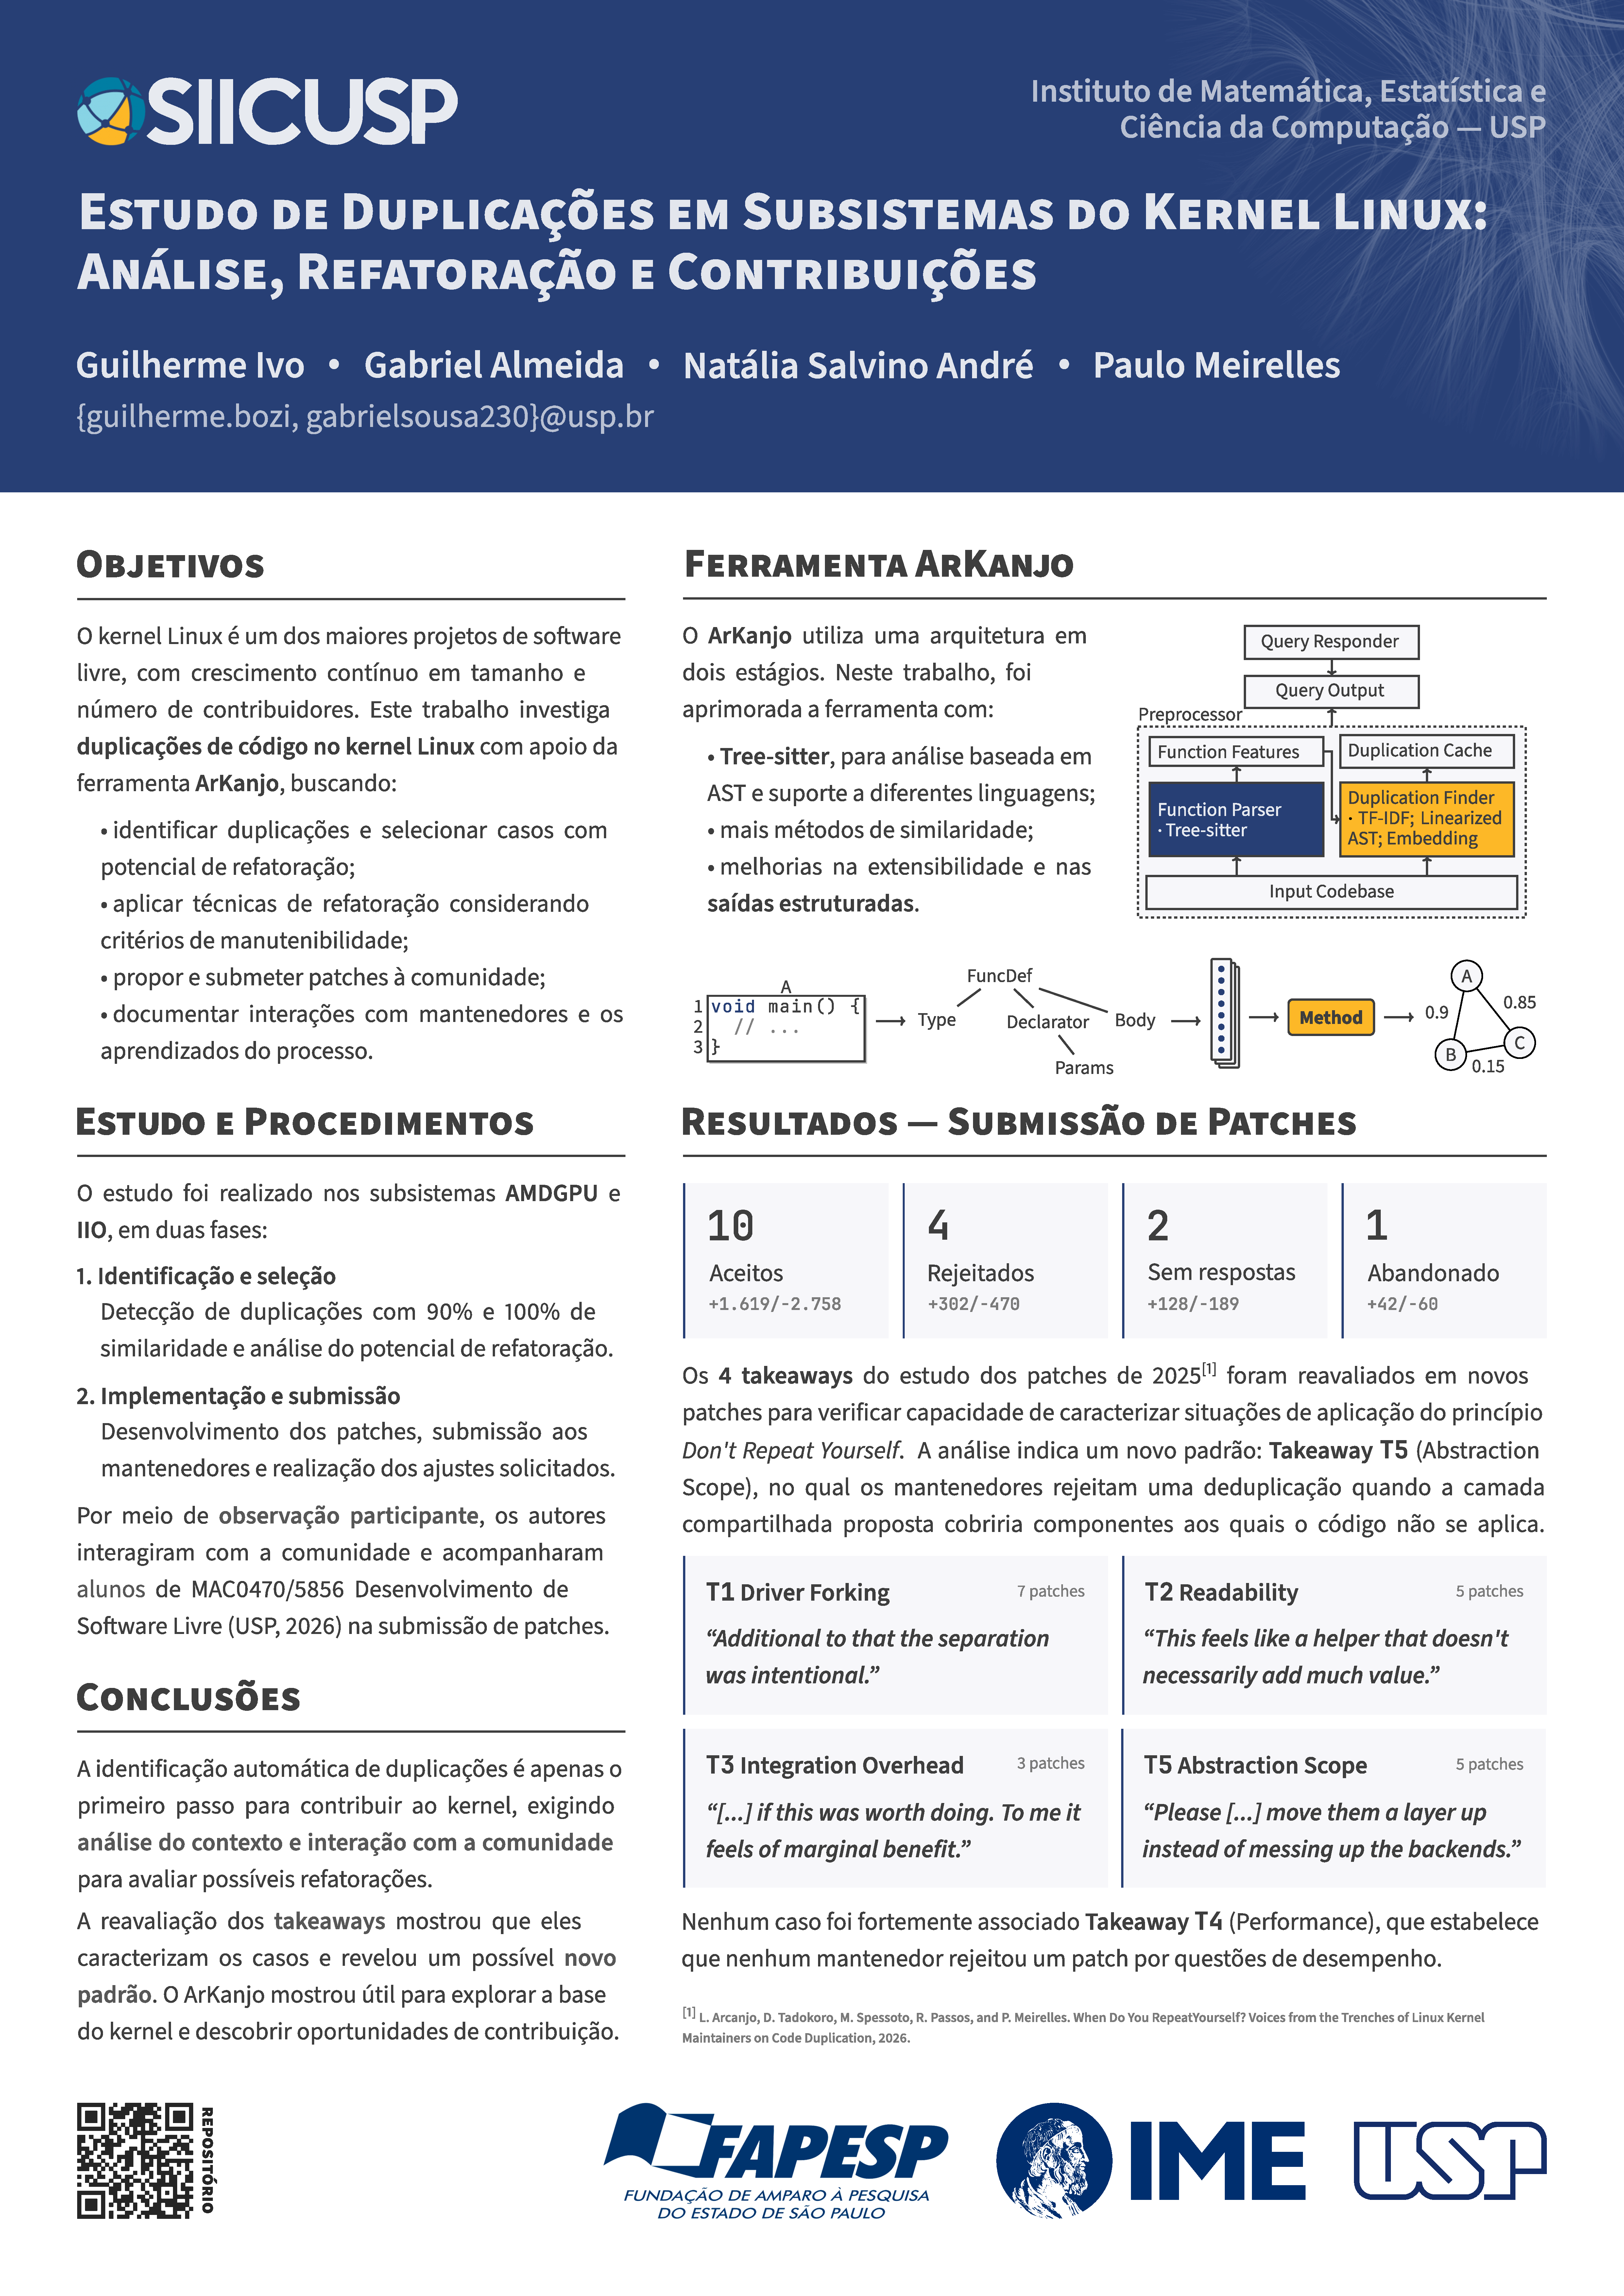
\includepdf[
    pages=-,
    scale=0.9,
    picturecommand={
        \color{black}
        \linethickness{0.5pt}
        \put(25,25){\framebox(545,790){}}
    }
]{figures/poster-siicusp.pdf}

% Para as publicações listadas no item 5, inclua cópias das primeiras páginas.

\section{Lista das publicações resultantes da bolsa}\label{apx:publicacoes-resultantes-da-bolsa}

{
\renewcommand{\newpage}{}
\renewcommand{\clearpage}{}
\renewcommand{\section}[2]{}

\bibliographystylepub{abnt}
\bibliographypub{references}
}

\subsection{Cópias das primeiras páginas das publicações}

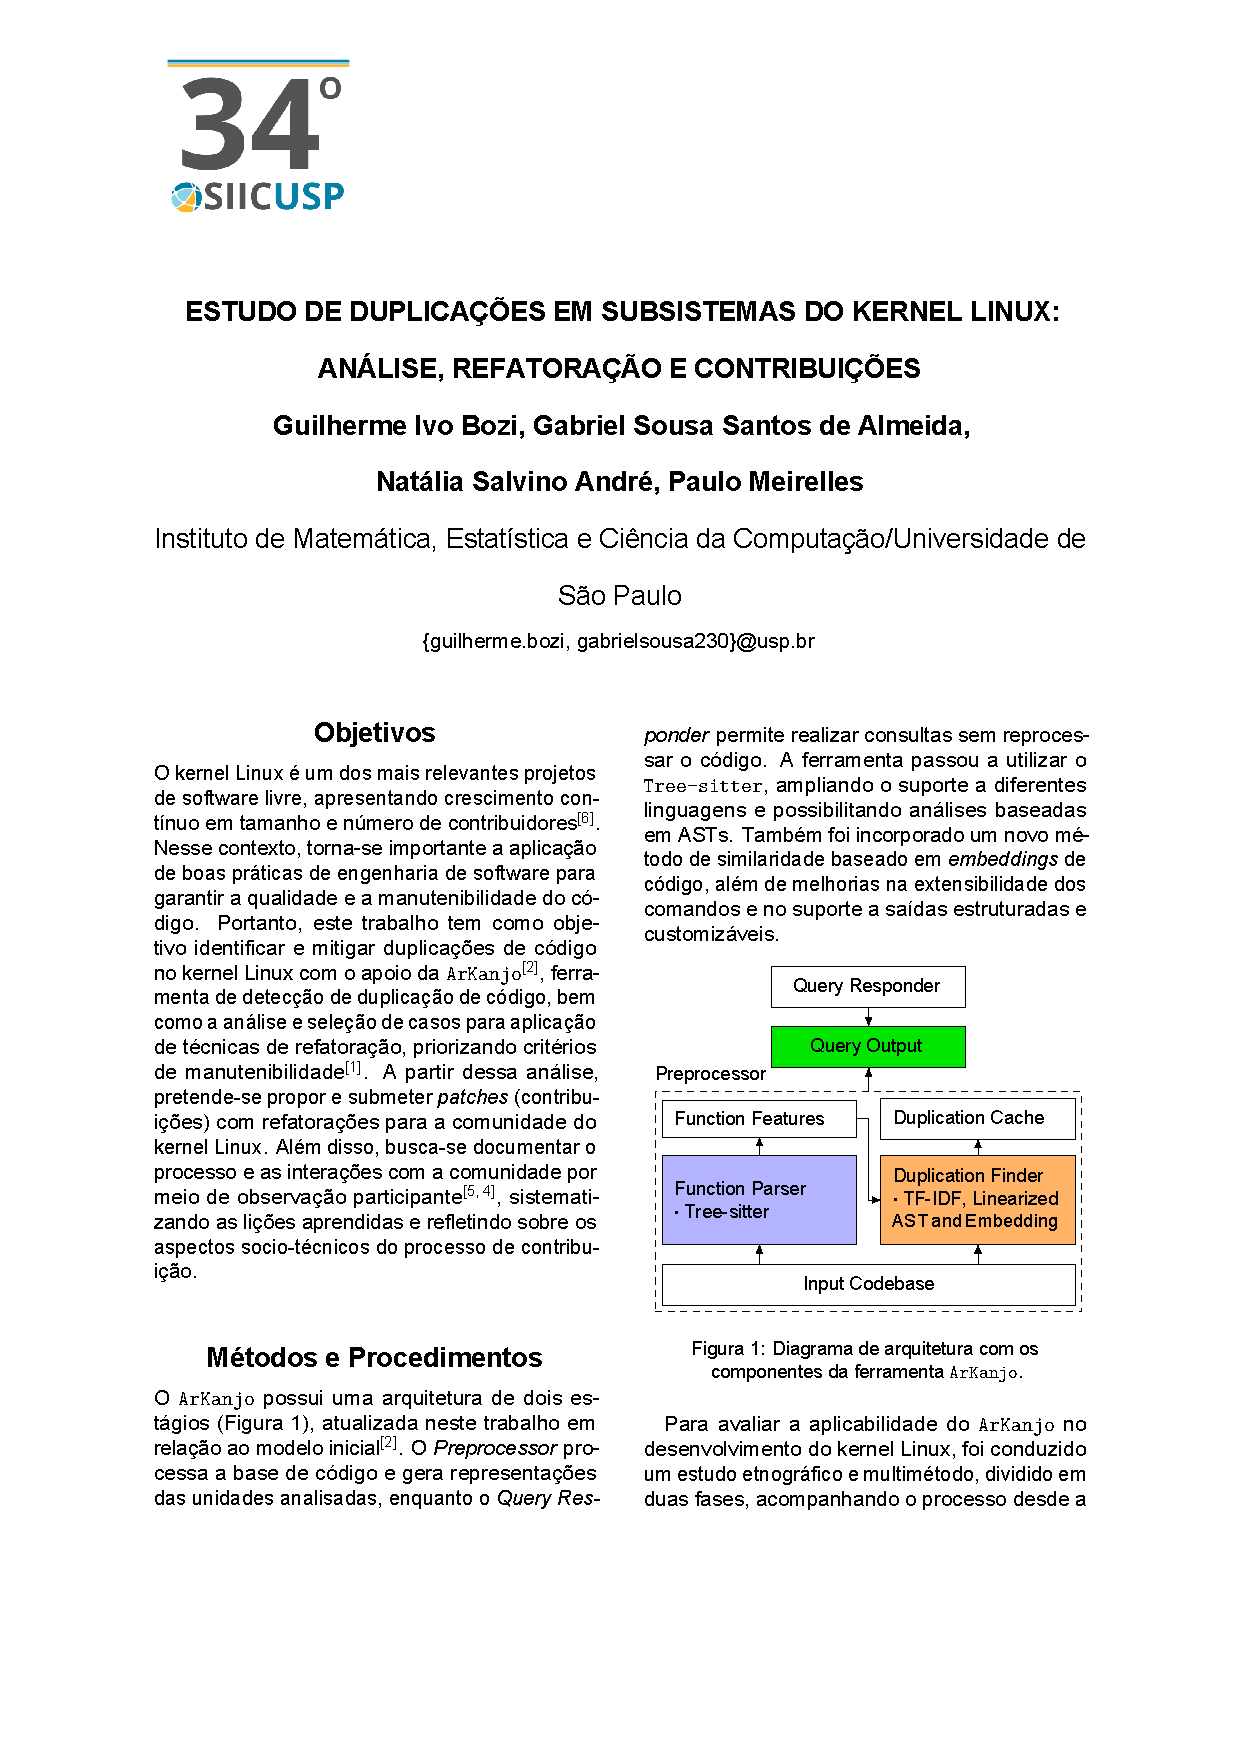
\includepdf[
    pages=-1,
    scale=0.9,
    picturecommand={
        \color{black}
        \linethickness{0.5pt}
        \put(25,25){\framebox(545,790){}}
    }
]{figures/abstract-siicusp.pdf}

\section{Lista dos trabalhos preparados ou submetidos, mas ainda não aceitos}\label{apx:trabalhos-em-preparacao}

Estão sendo preparados, em conjunto com o grupo de pesquisa, trabalhos científicos relacionados à análise de duplicações de código no kernel Linux e às ferramentas desenvolvidas no projeto. Esses trabalhos têm como objetivo divulgar os resultados obtidos e contribuir para a pesquisa na área de engenharia de software.

\begin{enumerate}
\item \textbf{TechDebt 2027 -- \textit{Short paper}:} Está em preparação um \textit{short paper} para submissão à International Conference on Technical Debt (TechDebt 2027), como extensão do trabalho \textit{``When Do You Repeat Yourself? Voices from the Trenches of Linux Kernel Maintainers on Code Duplication''}\cite{duplicationdry}. O estudo investiga as estratégias de deduplicação adotadas em séries de \textit{patches} relacionadas à remoção de duplicações de código, incluindo aquelas analisadas no trabalho anterior e novas contribuições obtidas no contexto de atividades acadêmicas recentes. O objetivo é caracterizar essas estratégias e identificar padrões e aprendizados sobre as abordagens utilizadas para eliminar duplicações, complementando a análise anterior, que se concentrou principalmente nos motivos para a rejeição de \textit{patches} (\textit{takeaways}).

\item \textbf{MSR 2027 -- \textit{Data and Tool Showcase Track}:} Está em preparação um artigo com foco na apresentação de um conjunto de dados relacionado à análise de duplicações de código no kernel Linux, construído a partir de um subconjunto do \textit{dataset} LKML5Ws\cite{passos2026lkml5ws}. O artigo pretende descrever o processo de construção do conjunto de dados, sua organização e suas possibilidades de utilização em pesquisas futuras, contribuindo para a reprodutibilidade e para novas investigações sobre duplicação de código no kernel Linux.
\end{enumerate}

Na data de elaboração deste relatório, ambos os trabalhos encontram-se em preparação para submissão e ainda não foram aceitos para publicação.

%TODO: colocar a versão inicial do techdebt2027, pode ser apenas a primeira página, com o abstract

\end{appendixenv}

\end{document}
